% \subsection{forms/src}
\subsection{forms/src}

% The @angular/forms/src directory contains these files:

@angular/forms/src 目录包含如下文件:

\begin{itemize}
  \item directives.ts
  \item form\_builder.ts
  \item form\_providers.ts
  \item forms.ts
  \item model.ts
  \item validators.ts
\end{itemize}

% forms\_providers.ts defines the
% \texttt{FormsModule}
% and
% \texttt{ReactiveFormsModule}
% NgModules as
% follows:

forms\_providers.ts 定义了 \texttt{FormsModule} 和 \texttt{ReactiveFormsModule} 两个 NgModules,
内容如下:

\begin{minted}{typescript}
@NgModule({
  declarations: TEMPLATE_DRIVEN_DIRECTIVES,
  providers: [RadioControlRegistry],
  exports: [InternalFormsSharedModule, TEMPLATE_DRIVEN_DIRECTIVES],
})
export class FormsModule {}
@NgModule({
  declarations: [REACTIVE_DRIVEN_DIRECTIVES],
  providers: [FormBuilder, RadioControlRegistry],
  exports: [InternalFormsSharedModule, REACTIVE_DRIVEN_DIRECTIVES],
})
export class ReactiveFormsModule {}
\end{minted}


% We note the two difference between
% \texttt{FormsModule}
% and
% \texttt{ReactiveFormsModule}
% are that
% \texttt{ReactiveFormsModule}
% has an additional
% \texttt{FormBuilder}
% provider configuration, and the
% export from
% \texttt{FormModule}
% includes
% \texttt{TEMPLATE\_DRIVEN\_DIRECTIVES}
% whereas the export
% from
% \texttt{ReactiveFormsModule}
% includes
% \texttt{REACTIVE\_DRIVEN\_DIRECTIVES}
% .

我们注意到 \texttt{FormsModule} 和 \texttt{ReactiveFormsModule} 两者的主要区别是:
\texttt{ReactiveFormsModule} 有一个额外的 \texttt{FormBuilder} provider 配置,
\texttt{FormModule} 的导出包含了 \texttt{TEMPLATE\_DRIVEN\_DIRECTIVES},
而 \texttt{ReactiveFormsModule} 的导出则包含 \texttt{REACTIVE\_DRIVEN\_DIRECTIVES}。

% directives.ts defines these:

directives.ts 定义如下:

\begin{minted}{typescript}
export const SHARED_FORM_DIRECTIVES: Type<any>[] = [
  NgSelectOption,
  NgSelectMultipleOption,
  DefaultValueAccessor,
  NumberValueAccessor,
  CheckboxControlValueAccessor,
  SelectControlValueAccessor,
  SelectMultipleControlValueAccessor,
  RadioControlValueAccessor,
  NgControlStatus,
  NgControlStatusGroup,
  RequiredValidator,
  MinLengthValidator,
  MaxLengthValidator,
  PatternValidator,
];
export const TEMPLATE_DRIVEN_DIRECTIVES: Type<any>[] = [
  NgModel,
  NgModelGroup,
  NgForm,
];
export const REACTIVE_DRIVEN_DIRECTIVES: Type<any>[] = [
  FormControlDirective,
  FormGroupDirective,
  FormControlName,
  FormGroupName,
  FormArrayName,
];
export const FORM_DIRECTIVES: Type<any>[][] = [
  TEMPLATE_DRIVEN_DIRECTIVES,
  SHARED_FORM_DIRECTIVES,
];
export const REACTIVE_FORM_DIRECTIVES: Type<any>[][] = [
  REACTIVE_DRIVEN_DIRECTIVES,
  SHARED_FORM_DIRECTIVES,
];

@NgModule({
  declarations: SHARED_FORM_DIRECTIVES,
  exports: SHARED_FORM_DIRECTIVES,
})
export class InternalFormsSharedModule {}
\end{minted}


% A nice discussion of how to create dynamic forms using
% \texttt{REACTIVE\_FORM\_DIRECTIVES}
% is here:

一个比较好的关于如何使用 \texttt{REACTIVE\_FORM\_DIRECTIVES} 创建动态表单的讨论:

\begin{itemize}
  \item \url{https://angular.io/docs/ts/latest/cookbook/dynamic-form.html}
\end{itemize}

% The form\_builder.ts file defines the injectable
% \texttt{FormsBuilder}
% class, which can
% dynamically construct a
% \texttt{FormGroup, FormArray}
% or
% \texttt{FormControl}
% via its
% \texttt{group()}
% ,
% \texttt{array()}
% or
% \texttt{control()}
% methods. They are defined as:

form\_builder.ts 文件定义了可注入的 \texttt{FormsBuilder} 类,
可以通过 \texttt{group()}、\texttt{array()} 或 \texttt{control()} 方法
动态构建相应的 \texttt{FormGroup}、\texttt{FormArray} 以及 \texttt{FormControl}。
方法定义如下:

\begin{minted}{typescript}
  group(
    controlsConfig: { [key: string]: any },
    extra: { [key: string]: any } = null
  ): FormGroup {
    const controls = this._reduceControls(controlsConfig);
    const validator: ValidatorFn = isPresent(extra)
      ? StringMapWrapper.get(extra, 'validator')
      : null;
    const asyncValidator: AsyncValidatorFn = isPresent(extra)
      ? StringMapWrapper.get(extra, 'asyncValidator')
      : null;
    return new FormGroup(controls, validator, asyncValidator);
  }

  control(
    formState: Object,
    validator: ValidatorFn | ValidatorFn[] = null,
    asyncValidator: AsyncValidatorFn | AsyncValidatorFn[] = null
  ): FormControl {
    return new FormControl(formState, validator, asyncValidator);
  }

  array(
    controlsConfig: any[],
    validator: ValidatorFn = null,
    asyncValidator: AsyncValidatorFn = null
  ): FormArray {
    var controls = controlsConfig.map((c) => this._createControl(c));
    return new FormArray(controls, validator, asyncValidator);
  }
\end{minted}


% The validators.ts file first declares two opaque tokens for dependency injection:

validators.ts 文件首先声明了两个用于依赖注入的 opaque tokens:

\begin{minted}{typescript}
export const NG_VALIDATORS: OpaqueToken = new OpaqueToken('NgValidators');
export const NG_ASYNC_VALIDATORS: OpaqueToken = new OpaqueToken(
  'NgAsyncValidators'
);
\end{minted}


% It also defines the Validators class:

它还定义了 Validators 类:

\begin{minted}{typescript}
// A validator is a function that processes a FormControl or
// collection of controls and returns a map of errors.
//
// A null map means that validation has passed.

export class Validators {
  static required(control: AbstractControl): { [key: string]: boolean } {}
  static minLength(minLength: number): ValidatorFn {}
  static maxLength(maxLength: number): ValidatorFn {}
  static pattern(pattern: string): ValidatorFn {}
}
\end{minted}


% A sample implementation of one of the validators is:

其中一个校验器的实现:

\begin{minted}{typescript}
  static required(control: AbstractControl): { [key: string]: boolean } {
    %\step{1}%
    return;
    %\step{2}% isBlank(control.value) ||
    (isString(control.value) && control.value == '')
      ? %\step{3}% { required: true }
      : %\step{4}% null;
  }
\end{minted}


% The return value
% 1
% is a string to boolean map. If the first line
% 2
% is true, then
% {'required': true} is returned
% 3
% , otherwise null
% 4
% is returned.

返回值 \step{1} 是一个 key 为 string,value 为 bool 的对象。
如果 \step{2} 处成立,则返回 \ts{{'required': true}} \step{3},
否则返回 null \step{4}。

% The model.ts file is large and defines the form control hierarchy:

model.ts 文件比较大,定义了表单控件继承关系(\fref{fig:form_control_hierarchy})。

\begin{figure}[!hbt]
  \centering
  \caption{Form Control Hierarchy}
  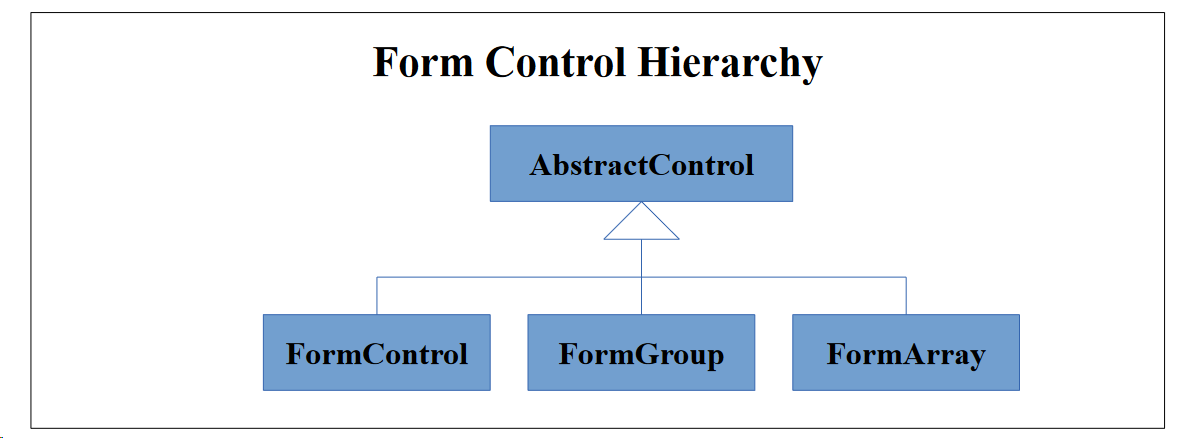
\includegraphics[width=0.75\linewidth]{15_the_forms_package/form_control_hierarchy}
  \label{fig:form_control_hierarchy}
\end{figure}

% The status of a form control is one of:

表单控件的状态是以下之一:

\begin{minted}{typescript}
// Indicates that a FormControl is valid,
// i.e. that no errors exist in the input value
export const VALID = 'VALID';

// Indicates that a FormControl is invalid,
// i.e. that an error exists in the input value.
export const INVALID = 'INVALID';

// Indicates that a FormControl is pending, i.e. that async validation is
// occurring and errors are not yet available for the input value.
export const PENDING = 'PENDING';

// Indicates that a FormControl is disabled, i.e. that the control is
// exempt from ancestor calculations of validity or value.
export const DISABLED = 'DISABLED';
\end{minted}


% The
% \texttt{AbstractControl}
% class defines a constructor, that takes in validator and async
% validator functions. This class also defines a bunch of getters which map to private
% fields. The value field refers to data we wish to strore within the control:

\texttt{AbstractControl} 类构造器接收一个 validator 和 async validator 函数。
还定义了一系列的 getters 用于映射私有字段。
value 字段代表我们想要存储在表单控件内的数据:

\begin{minted}{typescript}
  get value(): any {
    return this._value;
  }
\end{minted}


% The
% \texttt{\_status}
% field refers to the validator checking:

\texttt{\_status} 字段表示 validator 状态:

\begin{minted}{typescript}
  get status(): string {
    return this._status;
  }
  get valid(): boolean {
    return this._status === VALID;
  }
  get invalid(): boolean {
    return this._status === INVALID;
  }
  get pending(): boolean {
    return this._status == PENDING;
  }
\end{minted}


% The
% \texttt{\_error}
% field returns a map of errors (if any):

\texttt{\_error} 字段返回错误映射(如果有):

\begin{minted}{typescript}
  get errors(): { [key: string]: any } {
    return this._errors;
  }
\end{minted}


% The
% \texttt{\_pristine}
% field refers to whether the control’s data has been changed –
% \texttt{pristine()}
% is true if unchanged, and
% \texttt{dirty()}
% is true if changed:

\texttt{\_pristine} 字段代表控件数据是否改变了 —— \texttt{pristine()} 为 true 则表示未变化,
\texttt{dirty()} 为 true 则表示变化了:

\begin{minted}{typescript}
  get pristine(): boolean {
    return this._pristine;
  }
  get dirty(): boolean {
    return !this.pristine;
  }
\end{minted}


% The
% \texttt{\_touched}
% field refers to whether the user has visited the control (if does not
% mean that the control’s value has been changed):

\texttt{\_touched} 代表控件是否被用户访问(但这并不意味着控件值发生了变化)

\begin{minted}{typescript}
  get touched(): boolean {
    return this._touched;
  }
  get untouched(): boolean {
    return !this._touched;
  }
\end{minted}


% There are also two
% \texttt{xxChanges()}
% getters, for value changes and status changes, that
% return observables:

还有两个 \texttt{xxChanges()} getter,value changes 和 status changes,
返回 observables:

\begin{minted}{typescript}
  get valueChanges(): Observable<any> {
    return this._valueChanges;
  }
  get statusChanges(): Observable<any> {
    return this._statusChanges;
  }
\end{minted}


% These are initialized to event emitters via:

通过 event emitters 进行初始化:

\begin{minted}{typescript}
  _initObservables() {
    this._valueChanges = new EventEmitter();
    this._statusChanges = new EventEmitter();
  }
\end{minted}


% \texttt{AbstractControl}
% also declares a function:

\texttt{AbstractControl} 还声明了一个函数:

\begin{minted}{typescript}
  abstract _anyControls(condition: Function): boolean;
\end{minted}


% which executes the condition function over the control and its children and return a
% boolean. This
% \texttt{\_anyControls}
% function is used in many helper methods to determine
% information about the control, e.g.:

它对控件及其子控件执行条件函数并返回一个布尔值。
\texttt{\_anyControls} 函数在许多辅助函数中用于确定有关控件的信息,例如:

\begin{minted}{typescript}
  _anyControlsHaveStatus(status: string): boolean {
    return this._anyControls(
      (control: AbstractControl) => control.status == status
    );
  }
\end{minted}


% It has a parent field:

它有一个 parent 字段:

\begin{minted}{typescript}
  private _parent: FormGroup | FormArray;
\end{minted}


% which is used when the state of the control is being updated.

当控件的状态正在更新时使用。

\begin{minted}{typescript}
  markAsDirty({ onlySelf }: { onlySelf?: boolean } = {}): void {
    onlySelf = normalizeBool(onlySelf);
    this._pristine = false;
    if (isPresent(this._parent) && !onlySelf) {
      this._parent.markAsDirty({ onlySelf: onlySelf });
    }
  }
\end{minted}


% It is set via:

它通过以下方式设置:

\begin{minted}{typescript}
  setParent(parent: FormGroup | FormArray): void {
    this._parent = parent;
  }
\end{minted}


% Its is hierarchical and this is supplied to find the root:

它是继承的,用于查找根:

\begin{minted}{typescript}
  get root(): AbstractControl {
    let x: AbstractControl = this;
    while (isPresent(x._parent)) {
      x = x._parent;
    }
    return x;
  }
\end{minted}


% The FormControl class is supplied for atomic controls (that do not contain any child
% controls).

FormControl 类是为原子控件(不包含任何子控件)提供的。

\begin{minted}{typescript}
// By default, a `FormControl` is created for every `<input>` or
// other form component.
export class FormControl extends AbstractControl {
  _onChange: Function[] = [];

  // Register a listener for change events.
  registerOnChange(fn: Function): void {
    this._onChange.push(fn);
  }
  ..
}
\end{minted}


% Its
% \texttt{\_value}
% field is set via
% \texttt{setValue()}
% method which reacts depending on the four
% optional booleans supplied:

它的 \texttt{\_value} 字段是通过 \texttt{setValue()} 方法设置的,
该方法根据给定的四个可选布尔值做出相应改动:

\begin{minted}{typescript}
  setValue(
    value: any,
    {
      onlySelf,
      emitEvent,
      emitModelToViewChange,
      emitViewToModelChange,
    }: {
      onlySelf?: boolean;
      emitEvent?: boolean;
      emitModelToViewChange?: boolean;
      emitViewToModelChange?: boolean;
    } = {}
  ): void {
    emitModelToViewChange = isPresent(emitModelToViewChange)
      ? emitModelToViewChange
      : true;
    emitViewToModelChange = isPresent(emitViewToModelChange)
      ? emitViewToModelChange
      : true;

    this._value = value;
    if (this._onChange.length && emitModelToViewChange) {
      this._onChange.forEach((changeFn) =>
        changeFn(this._value, emitViewToModelChange)
      );
    }
    this.updateValueAndValidity({ onlySelf: onlySelf, emitEvent: emitEvent });
  }
\end{minted}


% It has a
% \texttt{reset()}
% method to reset control data:

\texttt{reset()} 方法用于重置控件数据:

\begin{minted}{typescript}
  reset(
    formState: any = null,
    { onlySelf }: { onlySelf?: boolean } = {}
  ): void {
    this._applyFormState(formState);
    this.markAsPristine({ onlySelf });
    this.markAsUntouched({ onlySelf });
    this.setValue(this._value, { onlySelf });
  }
\end{minted}


% The FormGroup class extends AbstractControl:

FormGroup 类继承自 AbstractControl:

\begin{minted}{typescript}
export class FormGroup extends AbstractControl {
  ..
}
\end{minted}


% Its constructor’s first parameter defines a controls associative map (in constrast to
% FormArray):

它的构造函数的第一个参数定义了一个控件关联映射(与 FormArray 形成对比):

\begin{minted}{typescript}
  constructor(
    public controls: { [key: string]: AbstractControl },
    validator: ValidatorFn = null,
    asyncValidator: AsyncValidatorFn = null
  ) {
    super(validator, asyncValidator);
    this._initObservables();
    this._setParentForControls();
    this.updateValueAndValidity({ onlySelf: true, emitEvent: false });
  }
\end{minted}


% Controls can be registered with FormGroup via:

可以通过以下方式向 FormGroup 注册控件:

\begin{minted}{typescript}
  // Register a control with the group's list of controls.
  registerControl(name: string, control: AbstractControl): AbstractControl {
    if (this.controls[name]) return this.controls[name];
    this.controls[name] = control;
    control.setParent(this);
    return control;
  }
\end{minted}


% The values of all controls in the group may be set via:

group 中所有控件的值可以通过以下方式设置:

\begin{minted}{typescript}
  setValue(
    value: { [key: string]: any },
    { onlySelf }: { onlySelf?: boolean } = {}
  ): void {
    this._checkAllValuesPresent(value);
    StringMapWrapper.forEach(value, (newValue: any, name: string) => {
      this._throwIfControlMissing(name); %\step{1}%
      this.controls[name].setValue(newValue, { onlySelf: true });
    });
    this.updateValueAndValidity({ onlySelf: onlySelf });
  }
\end{minted}


% Note it throws an exception is any of the controls are missing
% 1
% .

请注意,如果缺少任何控件,它会引发异常 \step{1}。

% The FormArray class extends AbstractControl:

FormArray 类继承自 AbstractControl:

\begin{minted}{typescript}
export class FormArray extends AbstractControl {
  ..
}
\end{minted}


% Its constructor’s first parameter is simply an array:

它的构造函数的第一个参数只是一个数组:

\begin{minted}{typescript}
  constructor(
    public controls: AbstractControl[],
    validator: ValidatorFn = null,
    asyncValidator: AsyncValidatorFn = null
  ) {
    super(validator, asyncValidator);
    this._initObservables();
    this._setParentForControls();
    this.updateValueAndValidity({ onlySelf: true, emitEvent: false });
  }
\end{minted}


% It allows you to insert at the end of the array or at a given location, and to remove:

允许你在数组的末尾或给定位置进行插入,删除:

\begin{minted}{typescript}
  // Insert a new {@link AbstractControl} at the end of the array.
  push(control: AbstractControl): void {
    this.controls.push(control);
    control.setParent(this);
    this.updateValueAndValidity();
  }

  // Insert a new {@link AbstractControl} at the given `index` in the array.
  insert(index: number, control: AbstractControl): void {
    ListWrapper.insert(this.controls, index, control);
    control.setParent(this);
    this.updateValueAndValidity();
  }

  // Remove the control at the given `index` in the array.
  removeAt(index: number): void {
    ListWrapper.removeAt(this.controls, index);
    this.updateValueAndValidity();
  }
\end{minted}

